%
%  version 1, 2016-12-05
%
\documentclass[twocolumn,twoside]{svmultivs_br} %please do not change this line
\usepackage{graphicx}
\usepackage{url}
\usepackage[table]{xcolor}
\usepackage{tabularx}
\usepackage{bm}
\usepackage{lipsum}
%
% The contents of \title* are printed on the first page.
% The contents of \subtitle are printed below the title on the
% first page.  This keyword is optional.
% The contents of \titlerunning are printed on the other pages.
% This should be a short version of the title.
%
\title*{Norwegian Mapping Authority Analysis Center Biennial Report}
\subtitle{2017--2018}
\titlerunning{NMA AC 2017--2018 Report}
%
% Example:
% \title*{IVS Coordinating Center 2015---2016 Biennial Report}
% \titlerunning{IVS CC 2015---2016 Report}
%
% \subtitle may be used if there is not enough room in \title*.  
% Example:
% \title*{International VLBI Service Coordinating Center Biennial Report Submission}
% \subtitle{Work during 2015---2016}
% \titlerunning{IVS CC 2015---2016 Report}
%
\author{Ann-Silje Kirkvik}
\authorrunning{Kirkvik} % see comments below
\authoremails{ann-silje.kirkvik@kartverket.no}
\institute{Norwegian Mapping Authority (NMA)}
%
% \author and \institute keywords:
%
% Each number in \author refers to an institution with which the author is associated.
% The numbers should correspond to numbered institutions in the \institute keyword.
% If all authors are associated with only one institution (the same institution),
% then the numbers should be omitted from \author and \institute.
% If an author is associated with two or more institutions, multiple numbers may be
% used.
%
% The \institute key word must be a single line.
% Please separate institutions using \\ between each institution.
%
% \authorrunning keyword:
%
% For one author, please use \authorrunning{last_name_of_author},
% e.g., \authorrunning{Behrend}
% For two authors, please use \authorrunning{last_name_of_first_author and last_name_of_second_author}
% e.g., \authorrunning{Behrend and Baver}
% For three or more authors, please use \authorrunning{last_name_of_first_author et al.}
% e.g., \authorrunning{Behrend et al.}
%
% Examples
%
% \author{Dirk Behrend}
% \authorrunning{Behrend}
% \author_emails{dirk.behrend-1@nasa.gov}
% \institute{NVI, Inc.}
%
% \author{Karen Baver, Dirk Behrend}
% \authorrunning{Baver and Behrend}
% \author_emails{karen.d.baver@nasa.gov,dirk.behrend-1@nasa.gov}
% \institute{NVI, Inc.}
%
% \author{John Gipson~$^1$, David Eriksson~$^{1,2}$, Chopo Ma~$^3$}
% \authorrunning{Gipson et al.}
% \institute{1. NVI, Inc. \\ 2. Chalmers University of Technology \\ 3. Goddard Space Flight Center}
%
\component{NMA Analysis Center} 
%
% Examples:
%Mets\"ahovi Network Station
%NEOS Operation Center
%Bonn Correlator
%INAF Data Center
%IAA Analysis Center
%NICT Technology Development Center
%
% Exceptions are the coordinators, who should use
%IVS Analysis Coordinator
% etc.
%
% \ContactAuthorName, \ContactAuthorTelephone, and \ContactAuthorEmail 
% should be used to identify the preferred contact author.
%
\ContactAuthorName{Ann-Silje Kirkvik}
\ContactAuthorTelephone{+47 32118421}
\ContactAuthorEmail{ann-silje.kirkvik@kartverket.no}
%
\NumberofInstitutions{1}
\InstitutionPostAddress{1}{Postboks 600 Sentrum, 3507 Hønefoss}
\InstitutionCountry{1}{Norway}
\InstitutionWebPage{1}{http://www.kartverket.no}
%
% Example:
%
% \InstitutionPostAddress{1}{61 avenue de l'Observatoire, 75014 Paris}
% \InstitutionCountry{1}{France}
% \InstitutionWebPage{1}{http://www.obspm.fr}
%
\begin{document}  %please do not change this line
%
\maketitle   %please do not change this line
%
%\abstract{\lipsum[1]}
\abstract{During 2017 and 2018, the Norwegian Mapping Authority has continued the development of the analysis
software \textbf{Where} that was started in 2015. The goal is to be able to use this
software to analyze VLBI data and contribute to operational IVS products. Extensive testing of the software has been
performed by analyzing over 20 years of 24-hour sessions and submitting the solution to the IVS Combination Center for
comparison with other analysis centers. After seven submissions with intermediate corrections of detected problems,
\textbf{Where} finally produced results that were comparable to other analysis centers and were ready to be included in
the IVS combination. Once the quality of the results were verified, the next step was start regular operational
submissions to test timeliness and operational robustness. This activity is anticipated to continue throughout 2019. }

%
\section{General Information}
The Norwegian Mapping Authority (NMA) has been an Associate Analysis Center within the IVS since 2010. The analysis
center is operated by the Geodetic Institute at NMA with main offices in H\o nefoss, Norway. NMA is a governmental agency with approximately 800 employees
and the IVS activities at NMA are completely funded by the Norwegian government.

NMA is using the analysis software \textbf{Where}, which is developed at NMA. The goal is to be able to use this
software to analyze VLBI data and contribute to operational IVS products. \textbf{Where} is freely available as open
source at GitHub \footnote{https://kartverket.github.io/where}.
Currently, the released version of \textbf{Where} can process individual VLBI sessions. \textbf{Where}
relies on VGOSDB version 4 as input and for the moment, it only supports the S/X-legacy observations.

Development is underway to support SLR and various applications of GNSS data. In addition, a lot of the functionality in
\textbf{Where} has been separated into a library called \textbf{Midgard}, which is also available on GitHub under the
same license \footnote{https://kartverket.github.io/midgard}.

\section{Staff}
The Geodetic Institute at NMA has approximately 50 employees. Some of the responsibilities include maintaining the
national reference frame, geoid and height system. The Geodetic Institute also provides a network-RTK positioning
service and operates the VLBI station in Ny-\AA lesund.

The \textbf{Where} development team has lost a few members due to changes in priorities and resignations, but it has
also gained some resources. The current staff is summarized in table \ref{tab:staff}.

\begin{table}[htb!]
\caption{Where developers and users at NMA}
\begin{center}
\begin{tabularx}{\linewidth}{X|X}
\hline
Name  & Tasks \\
\hline
Laila L\o vh\o iden & System owner \\
Michael D\"ahnn & GNSS developer \\
Mohammed Ouassou & GNSS developer \\
Ingrid Fausk & SLR developer \\
Ann-Silje Kirkvik & VLBI developer \\
\AA smund Skj\ae veland & VLBI analyst \\
\hline
\end{tabularx}
\end{center}
\label{tab:staff}
\end{table}


\section{Current Status and Activities}
%+ release on github, motivation for that
%+ comparing sessions with CCIVS, ref proceedings IVS GM. + table from Sabine + plot of UT1-UTC?
%+ contract with IGN, workshop etc
%+ completed working version of Where, supports vgosdb
%+ Status: VLBI, SLR, GNSS

NMA has been working on the development of \textbf{Where} since August 2015. In spring 2017, the software demonstrated
the ability to calculate theoretical delays comparable to other software packages \cite{kirkvik2017}. This was done by
comparing results from \textbf{Where} with results obtained in the VLBI Analysis Software Comparison Campaign 2015
\cite{klopotek2016}.

By the beginning of 2018, all the building blocks needed to do a complete analysis of a VLBI session were completed, but
a lot of testing and validation remained \cite{kirkvik2018}.

At the 10th IVS General Meeting in Longyearbyen
\textbf{Where} was released as an open source software \cite{hjelle2018}. At the time there was still some problems to
solve before the results obtained with \textbf{Where} were reliable, but the General Meeting seemed like a suitable
arena for making the announcement. The choice of releasing \textbf{Where} as open source was twofold. For one, it would
enable greater transparency about how results obtained with \textbf{Where} actually are produced. Additionally, it opens
up the possibility for others outside NMA to contribute to the software.

Succeeding the General Meeting the testing and improvement of \textbf{Where} continued. After submitting a total of 6 solutions to the IVS Combination Center (CCIVS), \textbf{Where}
finally produced results that were ready for to be included in the combination. The 6th solution contained all 24 hour
sessions from the beginning of 2002 to the end of 2017.

However, the abrupt hardware failure of some critical components in the IVS production chain forced the transition from
NGS file format to the VGOSDB format for the VLBI observables. All submitted solutions up to this point were based the NGS
file format. Therefore, to test the VGOSDB format a 7th solution was analyzed and submitted to the CCIVS. The 7th
solution contained all 24 hour sessions from the beginning of 1994 to the end of 2018.

With the exception of some differences in the quality code flag for some observations for some older sessions the VGOSDB
data seemed to produce the same results as the NGS files. There were also some larger differences compared to the
combined solution in the parameter estimates for the older data (1994-2002) that was only included in the latest
solution (figure \ref{fig:dut1}). This should be investigated further. One possibility is that the same parameterization
was used for the whole dataset regardless of session geometry and might have an effect on the results before and after
R1s and R4s were introduced in 2002.

However, for newer sessions
\textbf{Where} v0.16.2 and higher seems to produce results that can be included in the IVS Combination. The statistics
of the Earth Orientation Parameters (EOP) for the 7th solution is summarized in table \ref{tbl:stat} and figure
\ref{fig:dut1} shows the value of UT1-UTC compared to the combination for the same solution.

In relation to the new antennas being built in Ny-\AA lesund (\cite{kupiszewski2019}), NMA and IGN (Spain) have a
“Memorandum of Understanding” where IGN develops the broadband receivers for the new antennas and NMA provides the
analysis software \textbf{Where} and some training to IGN. In November 2018, four people from IGN visited NMA in Oslo and a VLBI analysis workshop with
\textbf{Where} was held for a five days (figure \ref{fig:workshop}). IGN also plans to use \textbf{Where} to become an
analysis center.

\begin{figure*}[htbp!]
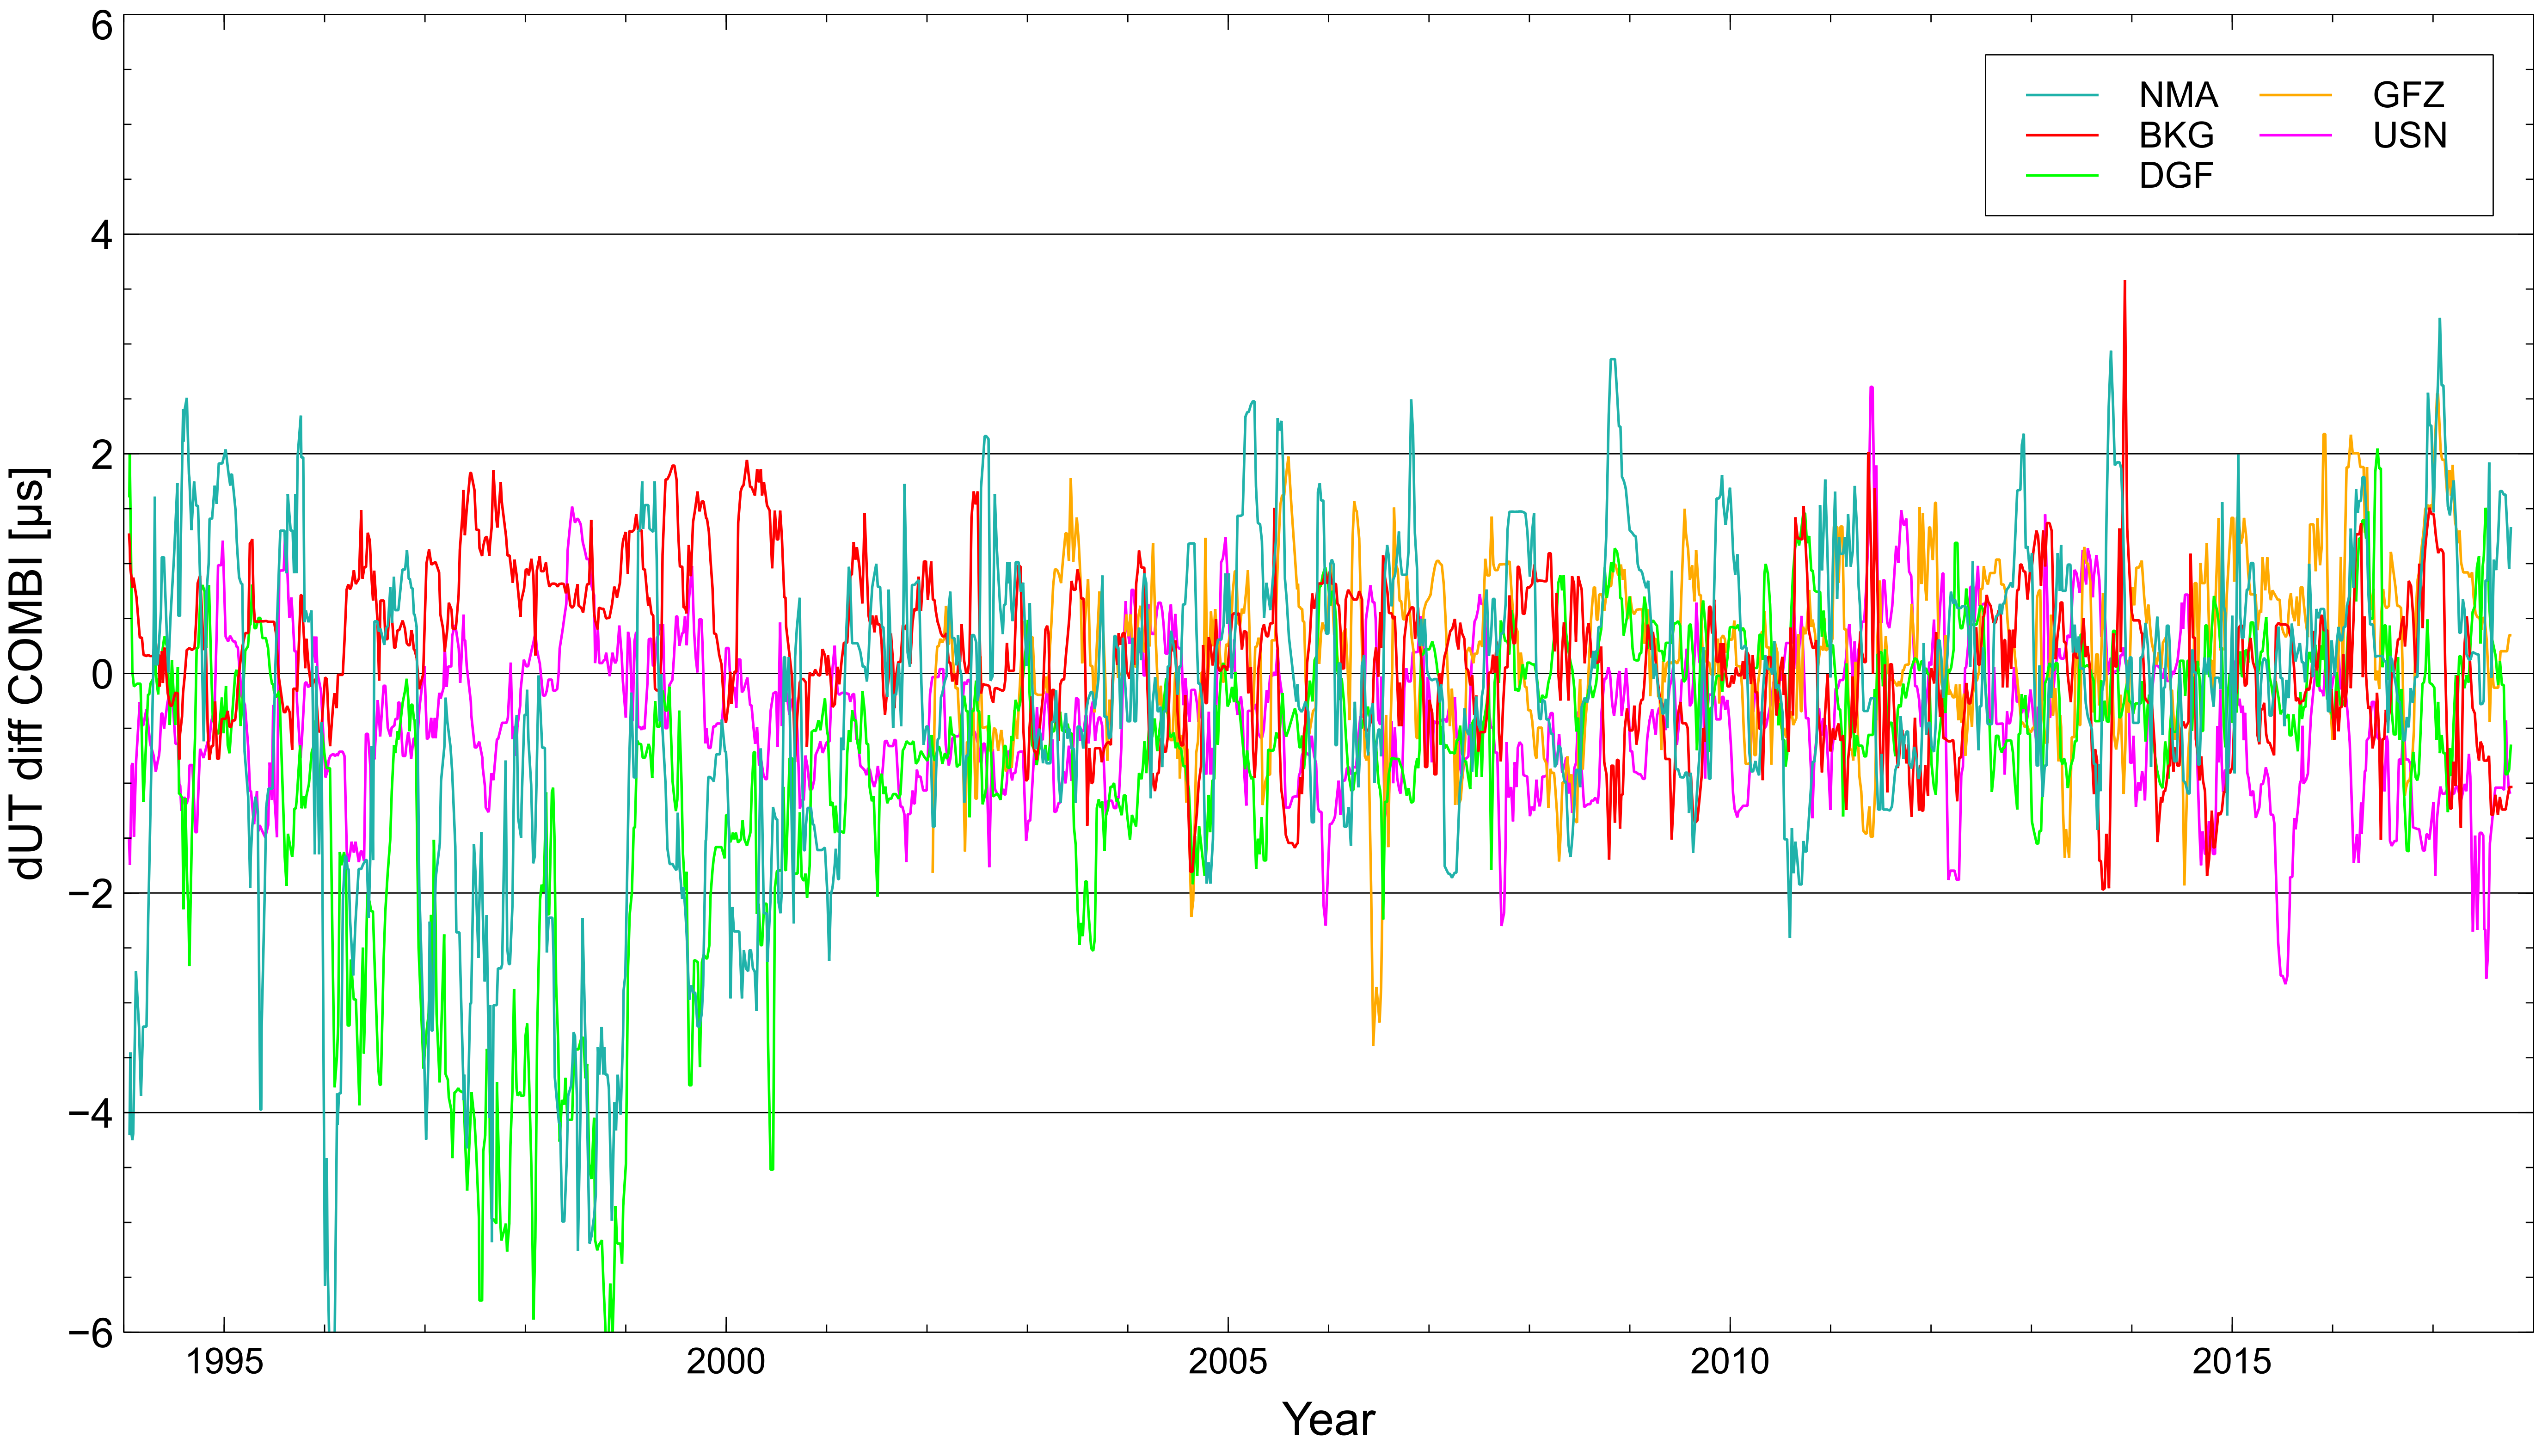
\includegraphics[width=\linewidth]{acnma01.png}
\caption{Difference between UT1-UTC and the combined solution for different analysis centers from the 7th solution.
Provided by Sabine Bachmann, BKG.}
\label{fig:dut1}
\end{figure*}

\begin{figure*}[htbp!]
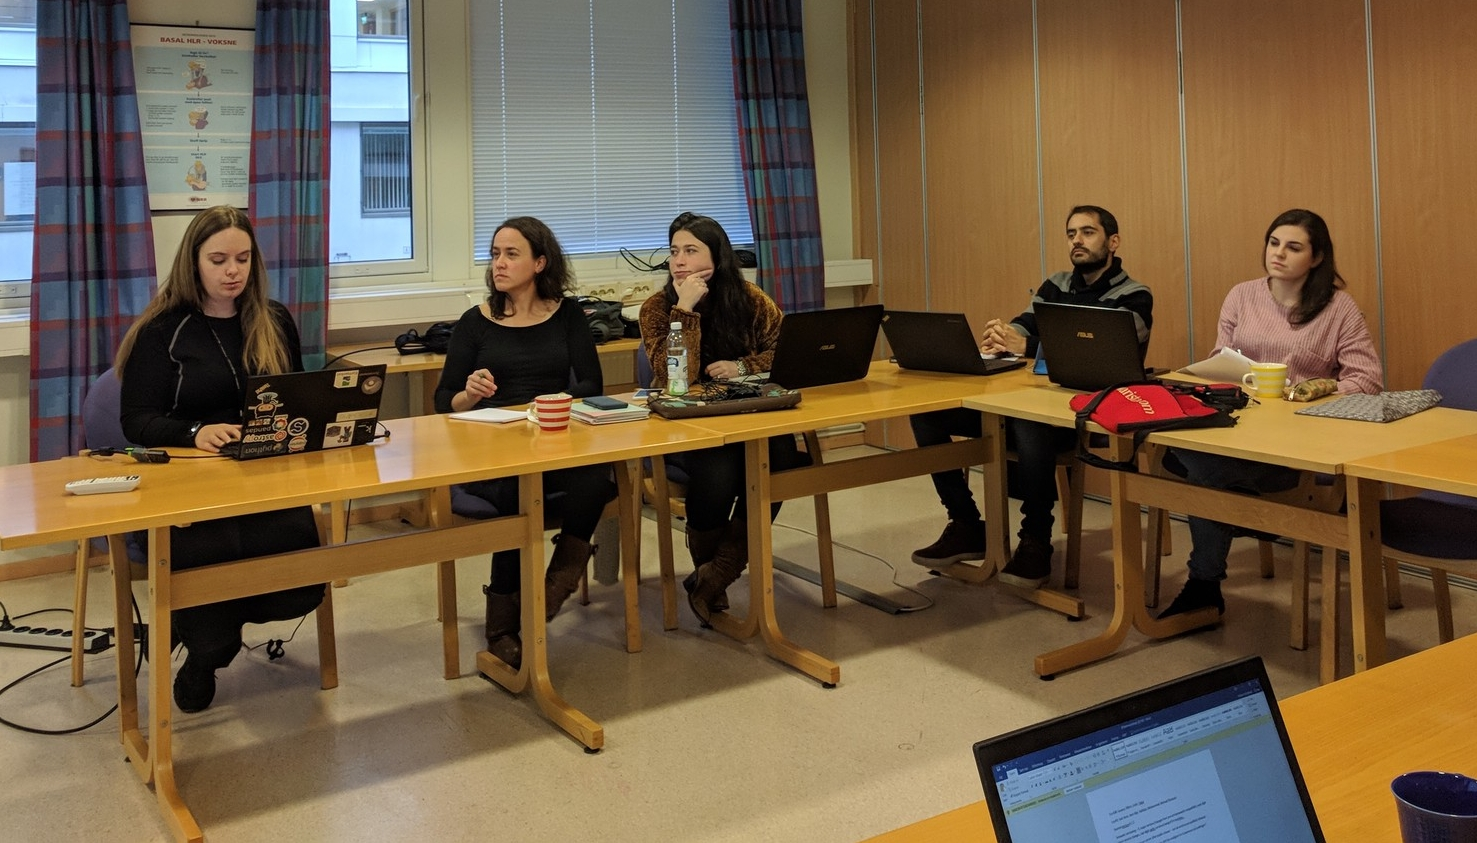
\includegraphics[width=\linewidth]{acnma02.jpg}
\caption{Workshop with IGN (Spain) at NMA offices in Oslo in November 2018. From the left:  Ann-Silje Kirkvik,
Susana Garcia Espada, Yaiza G\' omez Espada, Victor Puente, Esther Azcue. Photo:
Geir Arne Hjelle}
\label{fig:workshop}
\end{figure*}

\newcolumntype{L}{>{\raggedright\arraybackslash}X}
\newcolumntype{R}{>{\raggedleft\arraybackslash}X}
\begin{table*}[htbp!]
%\setlength\extrarowheight{10pt}
\caption{Statistics for a combined EOP solution for the eight EOP parameters: Polar motion $(x_p, y_p)$, Polar motion
rate $(\dot{x}_p, \dot{y}_p)$, UT1-UTC, Length of Day (LOD) and Celestial Pole Offset ($dX, dY$). Provided by Sabine
Bachmann, BKG.}
\begin{center}
\begin{tabularx}{\textwidth}{L|RRRRRR|RRRRRRR|}
\hline
\rowcolor{darkgray}
\multicolumn{1}{c}{\textbf{\color{white}AC}} & \multicolumn{1}{c}{\textbf{\color{white}WRMS}} &
\multicolumn{1}{c}{\textbf{\color{white}RMS}} & \multicolumn{1}{c}{\textbf{\color{white}Offset}} &
\multicolumn{1}{c}{\textbf{\color{white}Offset $\bm{\sigma}$}} & \multicolumn{1}{c}{\textbf{\color{white}Rate}} &
\multicolumn{1}{c}{\textbf{\color{white}Rate $\bm{\sigma}$}} & \multicolumn{1}{c}{\textbf{\color{white}WRMS}} &
\multicolumn{1}{c}{\textbf{\color{white}RMS}} & \multicolumn{1}{c}{\textbf{\color{white}Offset}} &
\multicolumn{1}{c}{\textbf{\color{white}Offset $\bm{\sigma}$}} & \multicolumn{1}{c}{\textbf{\color{white}Rate}} &
\multicolumn{1}{c}{\textbf{\color{white}Rate $\bm{\sigma}$}} \\
\hline\hline
& \multicolumn{6}{c|}{${x_p[\mu as]}$} & \multicolumn{6}{c|}{${y_p[\mu as]}$}  \\
\hline
 COMBI &  85.482 & 147.797 &  4.996 & 2.005 & -3.899 & 0.257 &  84.872 & 137.949 & 17.215 & 1.904 &  0.624 & 0.253 \\
   BKG & 104.468 & 167.126 & 12.367 & 2.247 & -4.980 & 0.301 & 102.267 & 159.001 & 19.341 & 2.140 &  0.880 & 0.293 \\
   ASI &   93.082 & 154.545 & 10.131 & 2.057 & -4.881 & 0.270 &  90.687 & 141.814 & 23.470 & 1.888 &  1.091 & 0.256\\
  DGFI &   64.588 & 178.511 & 36.369 & 2.256 & -5.143 & 0.305 &  57.148 & 141.185 &  0.466 & 1.977 & -0.715 & 0.270 \\
   GFZ &  100.864 & 171.606 &  8.712 & 2.367 & -7.669 & 0.454 &  99.952 & 173.951 & 13.286 & 2.283 &  0.075 & 0.454 \\
 GSFC  &   89.657 & 144.076 & 14.993 & 2.029 & -5.319 & 0.267 &  89.160 & 138.541 & 21.088 & 1.885 &  0.737 & 0.257 \\
 IAA   &  105.975 & 162.680 & 24.609 & 3.179 & -4.749 & 0.403 & 105.060 & 150.436 & 21.690 & 2.772 &  3.429 & 0.358 \\
 NMA &  112.984 & 234.652 & 21.267 & 2.385 & -6.474 & 0.336 & 113.388 & 414.675 & 15.222 & 2.295 & -0.391 & 0.337 \\
 OPA &   90.188 & 150.517 & 11.564 & 1.997 & -4.737 & 0.266 &  89.323 & 149.928 & 23.111 & 1.854 &  0.966 & 0.257\\
 USNO &   90.251 & 143.294 & 20.773 & 2.179 & -4.920 & 0.286 &  91.614 & 140.434 & 27.073 & 2.076 &  0.995 & 0.280 \\
 VIE&  213.394 & 247.003 & 25.398 & 6.620 & -4.159 & 1.303 & 178.649 & 213.642 & 21.028 & 5.347 &  3.994 & 1.089 \\
\hline\hline

& \multicolumn{6}{c|}{${\dot{x}_p[\mu as/d]}$} & \multicolumn{6}{c|}{${\dot{y}_p[\mu as/d]}$}
\\
\hline
 COMBI & 264.471 &  469.659 & -24.695 &  6.050 & -0.919 & 0.788 & 247.053 &  450.571 &   -8.792 &  5.451 &   1.947 &
 0.734 \\
 BKG & 325.188 &  566.456 & -39.181 &  7.290 &  1.910 & 0.961 & 310.450 &  537.123 &  -30.838 &  6.647 &   1.613 & 0.911
 \\
 ASI & 308.093 &  499.264 & -32.979 &  6.590 &  1.587 & 0.877 & 288.749 &  460.081 &  -14.195 &  5.948 &   1.098 & 0.817
 \\
 DGFI & 183.665 &  533.381 & -98.879 &  7.057 & -4.252 & 0.951 & 194.537 &  542.673 & -154.085 &  7.713 & -16.915 &
 1.045 \\
 GFZ & 319.974 &  501.040 & -20.847 &  7.511 &  2.294 & 1.465 & 316.942 &  647.830 &  -26.661 &  7.258 &  -1.871 & 1.461
 \\
 GSFC & 283.276 &  459.236 & -48.099 &  6.182 &  2.489 & 0.828 & 274.679 &  425.088 &  -22.325 &  5.753 &   1.654 &
 0.795 \\
 IAA & 308.771 &  465.454 & -73.600 &  8.691 &  3.182 & 1.095 & 315.316 &  435.988 &  -30.030 &  8.094 &   3.668 & 1.049
 \\
 NMA & 413.736 & 1688.182 & -14.232 &  8.724 & -1.461 & 1.219 & 389.543 & 1603.694 &  -52.370 &  7.899 &   5.033 & 1.147
 \\
 OPA & 303.316 &  549.385 & -43.161 &  6.477 &  2.196 & 0.878 & 286.488 &  554.111 &  -20.991 &  5.887 &   0.762 & 0.827
 \\
 USNO & 283.643 &  458.030 & -45.041 &  6.664 &  2.638 & 0.876 & 273.728 &  431.237 &  -20.899 &  6.169 &   1.777 &
 0.835 \\
 VIE & 522.554 &  764.064 &  18.635 & 15.751 & -4.356 & 3.230 & 524.599 &  820.935 &   31.969 & 16.131 &   8.995 & 3.219
 \\
\hline\hline
& \multicolumn{6}{c|}{${UT1-UTC[\mu s]}$} & \multicolumn{6}{c|}{${LOD[\mu s/d]}$}  \\
\hline
COMBI & 9.159 & 11.505 & -2.073 & 0.170 &  0.435 & 0.030 & 17.719 & 27.904 & -2.200 & 0.370 & 0.410 & 0.055 \\
  BKG &   9.455 & 11.856 & -2.482 & 0.175 &  0.428 & 0.031 & 19.590 & 29.297 & -0.925 & 0.393 & 0.139 & 0.059 \\
  ASI &   9.301 & 11.513 & -2.000 & 0.172 &  0.389 & 0.030 & 19.432 & 26.668 & -0.322 & 0.375 & 0.159 & 0.058 \\
 DGFI &   9.987 & 12.430 & -2.980 & 0.186 &  0.545 & 0.034 &  8.860 & 30.054 &  0.016 & 0.426 & 1.534 & 0.058 \\
  GFZ &   6.981 & 11.189 & -0.691 & 0.185 &  0.155 & 0.039 & 19.103 & 36.399 & -2.388 & 0.429 & 0.086 & 0.088 \\
 GSFC &   9.118 & 11.127 & -2.333 & 0.169 &  0.416 & 0.030 & 19.083 & 27.683 & -0.686 & 0.373 & 0.204 & 0.059 \\
 IAA  &  10.231 & 10.965 & -4.327 & 0.223 &  0.501 & 0.036 & 21.588 & 25.348 & -1.667 & 0.512 & 0.082 & 0.072 \\
 NMA  &  10.367 & 14.944 & -2.194 & 0.203 &  0.511 & 0.037 & 22.785 & 70.958 & -4.430 & 0.450 & 0.379 & 0.072 \\
 OPA &   9.199 & 12.245 & -2.385 & 0.171 &  0.416 & 0.030 & 19.479 & 31.390 & -0.518 & 0.378 & 0.210 & 0.059 \\
 USNO &   8.937 & 10.735 & -3.124 & 0.178 &  0.434 & 0.032 & 19.342 & 27.826 & -0.244 & 0.410 & 0.164 & 0.063 \\
  VIE &  15.821 & 16.683 & -0.944 & 0.515 & -0.003 & 0.101 & 56.137 & 63.877 & -1.526 & 1.609 & 0.228 & 0.344 \\
\hline\hline
& \multicolumn{6}{c|}{${dX[\mu as]}$} & \multicolumn{6}{c|}{${dY[\mu as]}$} \\
\hline
COMBI & 45.741 &  70.212 &  -5.969 & 0.963 & -2.202 & 0.128 & 40.390 &  80.073 &  1.771 & 0.862 & 1.777 & 0.114 \\
  BKG &  67.782 &  94.817 &  -6.517 & 1.413 & -2.870 & 0.191 & 61.826 & 100.966 &  0.188 & 1.308 & 2.666 & 0.175 \\
  ASI &  53.265 &  75.964 &  -8.905 & 1.075 & -1.367 & 0.145 & 49.918 &  88.444 &  2.044 & 1.017 & 1.650 & 0.137 \\
 DGFI &  40.674 & 105.057 & -19.264 & 1.418 & -5.223 & 0.192 & 34.031 & 106.957 &  0.566 & 1.223 & 1.328 & 0.165\\
  GFZ &  78.905 & 110.921 & -13.869 & 1.808 & -4.343 & 0.360 & 73.225 & 122.437 & 10.874 & 1.686 & 4.505 & 0.335 \\
 GSFC & 47.793 &  70.765 & -16.549 & 0.981 & -1.332 & 0.133 & 44.033 &  77.582 &  0.194 & 0.915 & 1.705 & 0.124\\
 IAA  &     NaN &     NaN &     NaN &   NaN &    NaN &   NaN &    NaN &     NaN &    NaN &   NaN &   NaN &   NaN\\
 NMA  &  94.091 & 221.678 & -17.820 & 1.863 & -3.208 & 0.264 & 91.552 & 214.698 &  7.402 & 1.837 & 3.001 & 0.260 \\
 OPA  &  48.586 &  86.868 &  -8.856 & 0.979 & -1.306 & 0.135 & 48.760 &  91.834 & -0.009 & 0.994 & 1.539 & 0.136 \\
 USNO &  52.302 &  68.892 &  18.141 & 1.157 & -2.195 & 0.154 & 46.457 &  65.989 &  9.763 & 1.042 & 0.639 & 0.139  \\
  VIE &  92.079 & 142.458 & -13.915 & 2.796 & -1.193 & 0.564 & 94.641 & 139.353 & -3.818 & 2.890 & 2.115 & 0.582 \\
\hline
\end{tabularx}
\end{center}
\label{tbl:stat}
\end{table*}


\section{Future Plans}
With the promising results from the testing period, NMA is now ready to try to contribute to the operational analyses.
The submission of regular timely analyses of R1 and R4 sessions will start at the beginning of 2019. NMA also plans to
contribute to the next realization of the international reference frame, namely ITRF2020.

The development of \textbf{Where} will also continue. Some possible extensions are to support analysis of VGOS data,
support VGOSDB version 1, better support for analysis of intensive sessions, support estimation of global solution
across multiple sessions, support different estimators or to look into further automation of the analysis. It is still
not decided which of these tasks should be prioritized.

\section*{Acknowledgements}

Thanks to Sabine Bachmann (BKG) at the IVS Combination Center for analyzing our solutions and providing
great feedback and insights.

\begin{thebibliography}{99}
\bibitem{hjelle2018}
Hjelle, G. A., et~al., Making Where available to the community, in Behrend, D., Baver, K.~D., Armstrong, K.~L.
(eds.), \emph{Global Geodesy and the Role of VGOS – Fundamental to Sustainable Development}, vol. NASA/CP-2018-?????? of \emph{IVS General
Meeting Proceedings}, pp. ???--???, IVS, 2018.

\bibitem{kirkvik2017}
Kirkvik, A.-S., et~al., Where - a new software for geodetic analysis, in Haas,
R., Elgered, G. (eds.), \emph{Proceedings of the 23rd European VLBI Group for
Geodesy and Astrometry Working Meeting}, 2017.

\bibitem{kirkvik2018}
Kirkvik, A.-S., et~al., {NMA} Analysis Center -- Progress Report, in Behrend, D., Baver, K.~D., Armstrong, K.~L. (eds.),
\emph{Global Geodesy and the Role of VGOS – Fundamental to Sustainable Development}, vol. NASA/CP-2018-?????? of \emph{IVS General
Meeting Proceedings}, pp. ???--???, IVS, 2018.

\bibitem{klopotek2016}
Klopotek, G., et~al., Results from the {VLBI} analysis software comparison
campaign 2015, in Behrend, D., Baver, K.~D., Armstrong, K.~L. (eds.),
\emph{New Horizons with VGOS}, vol. NASA/CP-2016-219016 of \emph{IVS General
Meeting Proceedings}, pp. 203--207, IVS, 2016.

\bibitem{kupiszewski2019}
Kupiszewski, P., Ny-\AA lesund Geodetic Observatory, in K. L. Armstrong, K. D. Baver, and D. Behrend (eds)
\emph{International VLBI Service for Geodesy and Astrometry 2017+2018 Biennial Report}, this volume.

\end{thebibliography}
%
\end{document}
